\chapter{Implementation of proposed methods}

This project is implemented by deep learning framework PyTorch and Py-Enigma library. PyTorch has become one of the most popular deep learning frameworks in academia because it fits the habits of Python users. It provides most of the neural network architecture (Linear, Convolutional, Recurrent, Transformer, etc), automatic differentiation, and toolkits for dataset, image, text, and audio processing. Py-Enigma is another Python library that simulates the Enigma behaviour. 

\section{Dataset}

\begin{figure}
    \centering
    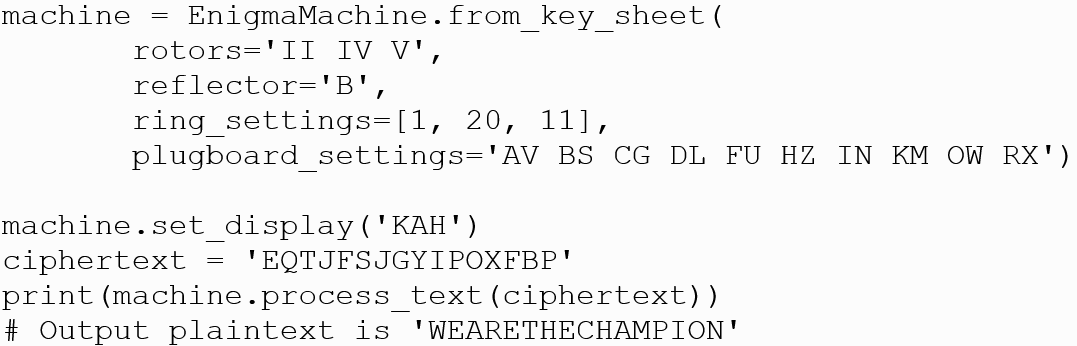
\includegraphics[width=0.8\linewidth]{myReport//figures/Enigma_pseudo.png}
    \caption{The pseudo code of how the Enigma Python API generate the data set in random}
    \label{fig:enter-label}
\end{figure}

To generate training data, we use an Enigma Python library to generate our training data. All plaintexts are generated randomly, then encrypted by the Py-Enigma library. The Py-Enigma provides the option to configure the number of rotors, ring setting of rotors, plugboard connection, and types of reflectors. This allows us to make our own customised Enigma machine, including Enigma with more than 5 rotors. The Py-enigma also requires an initial state input, which is also selected at random. By this method, we can generate an infinite amount of training data for our task. Below is a pattern of pseudocode of ciphering a plaintext sequence to ciphertext, showing how we can configure the Py-enigma API. Settings include, rotors, reflector, ring settings, plugboard, and initial positions.

In our task, which is attacking a three-rotor Enigma, we assume we know all the setting (Plugboard, ring settings, rotors type, Reflector types) except for initial states. So, we have 17576 different combinations of rotor positions. During training, for each training loop, we generate 200 samples for each possible initial state. It means that in a single training loop, we feed 1.7576e+6 samples into the neural networks. We used PyTorch Dataset API to generate pairs of plaintexts and ciphertext and stack multiple samples into mini batch. 

\begin{figure}[hbt!]
    \centering
    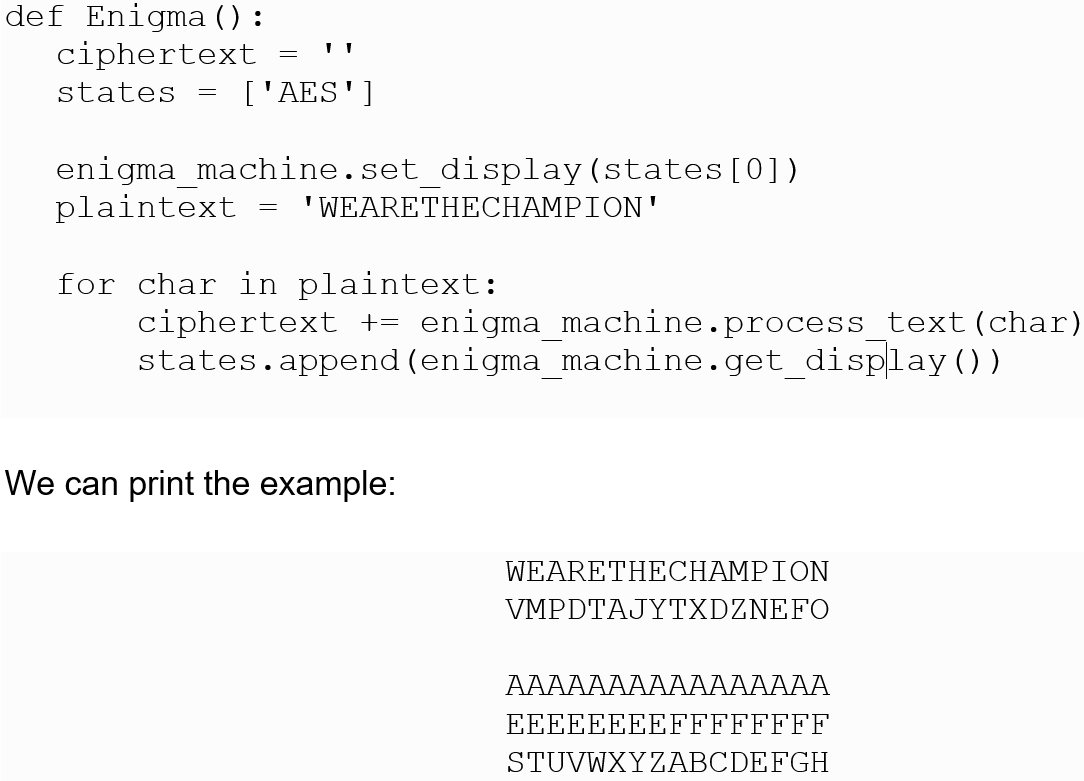
\includegraphics[width=0.6\linewidth]{myReport//figures/Dataset_pseudo.png}
    \caption{The pseudo code of data generation}
    \label{fig:enter-label}
\end{figure}

Py-Enigma’s get-display function returns the rotors current position. This allows us to generate ground truth for each pair of characters in ciphertext and plaintext, not just the initial state. The following pseudo code is an example of how the plaintexts are transfered to ciphertext and how we can get position for each step. We use plaintext ‘WEARETHECHAMPION’ and initial state ‘AES’ as examples here.

% \begin{figure}[hbt!]
%     \centering
%     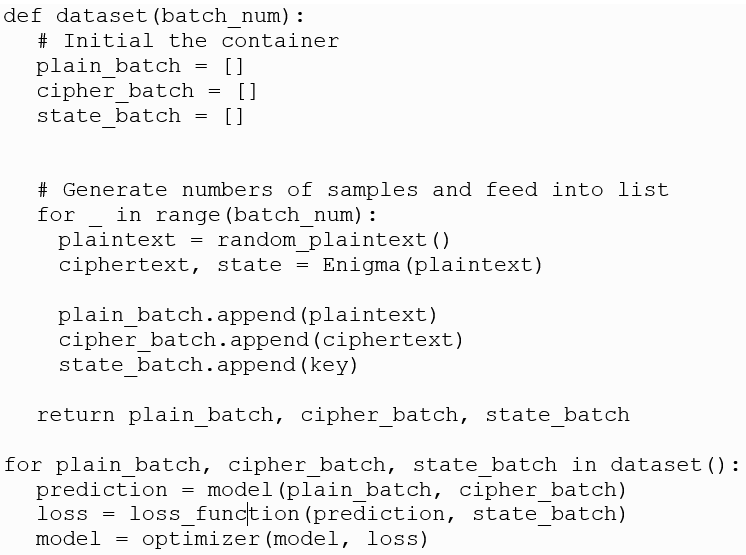
\includegraphics[width=0.7\linewidth]{myReport//figures/Dataset_pipeline.png}
%     \caption{The pseudo code of pipeline of training}
%     \label{fig:enter-label}
% \end{figure}

After dataset generated batched outputs, the training loop would feed batched plaintext and ciphertext into networks, compute the loss and optimize the networks. This pseudo code below shows the concept of how the network feedforward and optimized during training.


\section{Network architectures}
% \begin{figure}[hbt!]
%     \centering
%     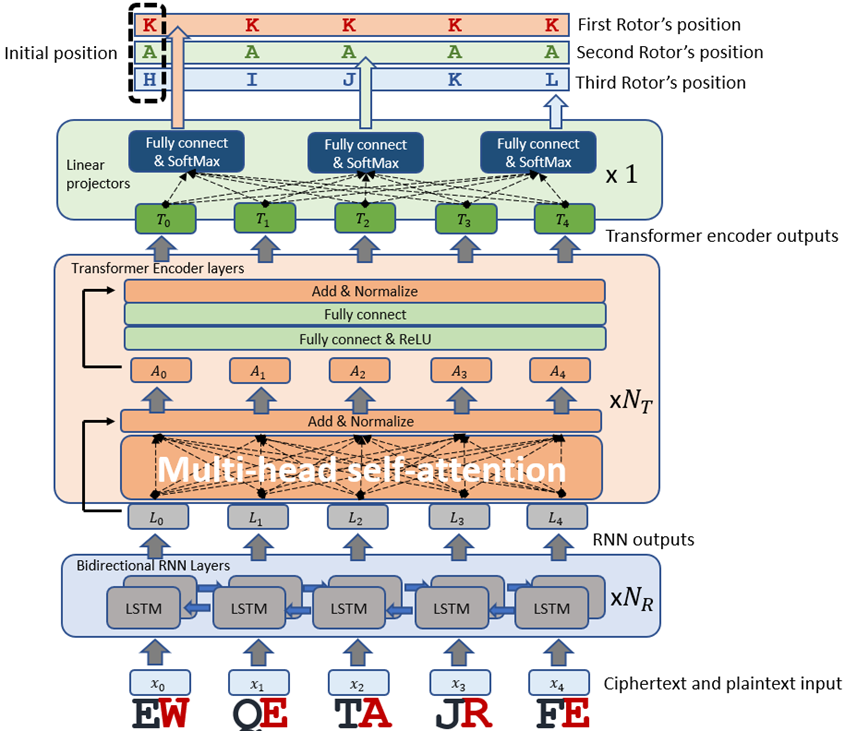
\includegraphics[width=0.85\linewidth]{myReport//figures/ours.png}
%     \caption{Enter Caption}
%     \label{fig:enter-label}
% \end{figure}
Like most neural networks, our network is a probabilistic model that predicts conditional probabilities for the rotor position for each input. Its function could be defined as: 

\begin{center}
\(p(R_1,R_2,R_3 |p_1,…p_n,c_1,…c_n)=Net(p_1,…p_n,c_1,…c_n)\) 
\end{center}

Where the \(R_n\) is the probabilities of 26 position of each rotors. \(p_n\) and \(c_n\) is the given plaintext and paired ciphertext. Net is the neural network model we used in this project. After the prediction, we would use Argmax, which also called a greedy search, to pick up the position with largest probability. The positions with maximum probability would be the final outputs of the network.


\begin{figure}[hbt!]
    \centering
    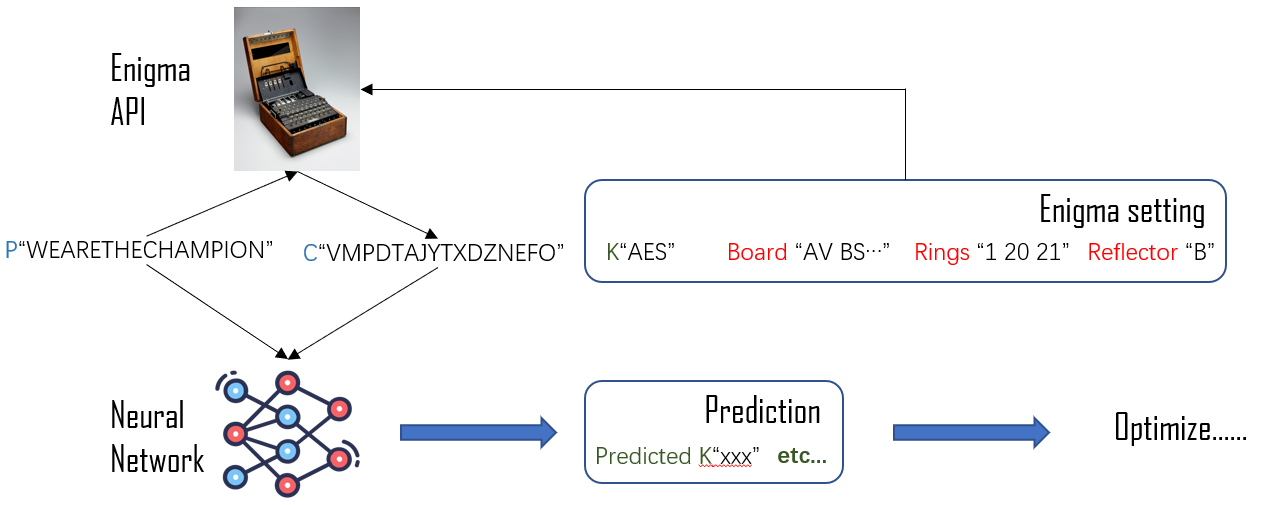
\includegraphics[width=0.8\linewidth]{myReport//figures/prototype.png}
    \caption{Data structure of our training pipeline}
    \label{fig:enter-label}
\end{figure}


\textbf{Figure 3.3} shows the prototype of our Entire project, include the neural network for prediction, the Enigma API for prediction. The “P” refer to the plain text we send into Python Enigma API, and the “C” is the cipher text computed based on plain text and all the content in Enigma setting. Plain text and cipher text would be fed into the neural network in pairs to make the prediction of content in Enigma setting. At the end, we use the Enigma setting as the supervised signal to optimize our network. We expected the network could achieve the attack by recovery of the content in Enigma setting by looking at the plain text and cipher text. Noticed that we would vary the difficulty and complexity by predicting different amount of Enigma setting. The setting would be initialized randomly but only apply to the setting we want to predict, the settings we don't need to predict would stay fixed or using the default setting. The example we showed in figure only make prediction on key bits(initial states), so the K would be randomly generate during the training, other settings like plugboard, ring settings, and reflector type would remain in default. 

\begin{figure}[hbt!]
    \centering
    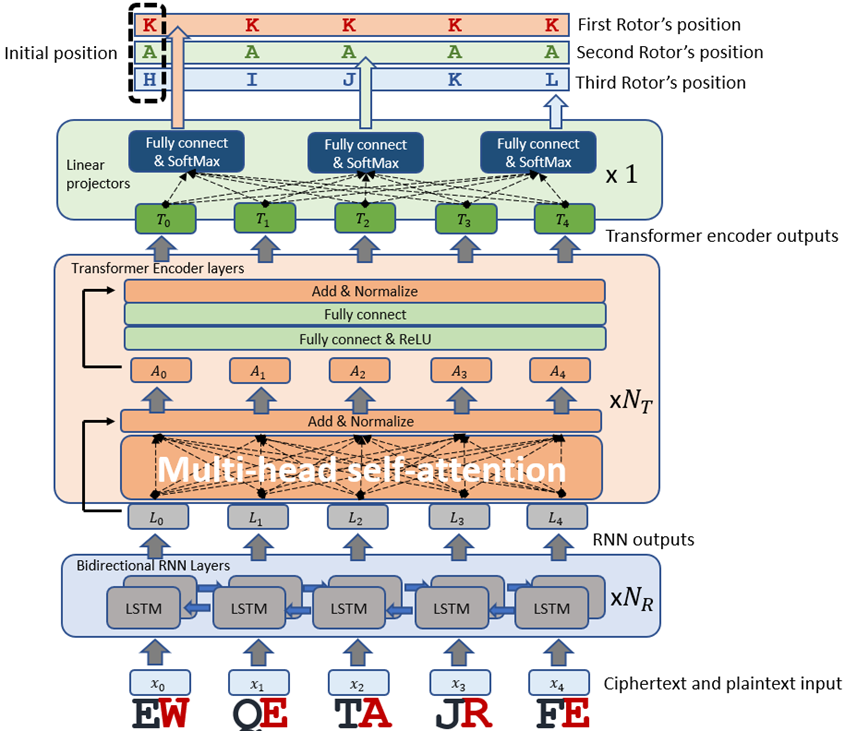
\includegraphics[width=1\linewidth]{myReport//figures/ours.png}
    \caption{Our hybrid models for machine learning cryptanalysis}
    \label{fig:enter-label}
\end{figure}

Our model is a combination of Long Short-Term Memory (LSTM) network layers, Transformer Encoder layers, and three to four linear projectors for final predictions. \textbf{Figure 3.4} shows a visualization of the architecture. We first transfer our input ciphertext and plaintext of length \(t\) into vectors \(x_t\). It could be one-hot encoding, or other forms of vectors. Then we have \(N_R\) layers of RNN layers and it will compute the RNN outputs \(L_t ( t=[0,1,…,t-1])\) by input features. Then the RNN outputs \(L_t\) will be feed into the Transformer Encoder layers to compute the outputs \(T_t\). Three fully connected layers would compute the final positions by a SoftMax activation. In our project we used three linear projectors because we are targeting the three rotors Enigma. It could be extended to 4 or more models of Enigma machines.

\noindent\textbf{Embedding layer} \qquad		In Natural language processing tasks, word embedding layers transfer words into their representation vectors. It usually implemented by a single linear layer. Takes the one-hot encoding of words as inputs and outputs the word vectors. 

% \begin{center}
% \(V_t=x_t W_\text{emb}\)
% \end{center}

In our attacking task, although we didn’t use words as inputs, but we still keep embedding layer as an initial layer to increase the channels and learnable parameters.

\noindent\textbf{LSTM layers} \qquad		The LSTM is the core function of our model because of its strong ability to model the time series relation between tokens. For each token in sequence, it computes the outputs depends on the current token, the previous token’s outputs, and its parameters. The computational function of each timestep could be defined as: 

\begin{center}
\(i_t=Sigmoid(W_\text{ii} x_t+ b_\text{ii}  +W_\text{hi} h_\text{t-1}+ b_\text{hi})\)
\\
\(f_t=Sigmoid(W_\text{if} x_t+ b_\text{if}  +W_\text{hf} h_\text{t-1}+ b_\text{hf})\)
\\\(g_t=TanH(W_\text{ig} x_t+ b_\text{ig}  +W_\text{hg} h_\text{t-1}+ b_\text{hg})\)
\\
\(O_t=Sigmoid(W_\text{io} x_t+ b_\text{io}  +W_\text{ho} h_\text{t-1}+ b_\text{ho})\)
\\
\(C_t=f_t \odot C_\text{t-1}+i_t \odot g_t\)
\\
\(h_t=O_t \odot TanH(C_t)\)
\\
\(L_t = \sum_{1}^{N_R} \sum_{t=0}^{n-1}h_t\)
\end{center}



These formulas are from PyTorch official documentation of LSTM. In this set of formula, \(x_t\) is the input of current sequence. \(h_t\) and \(h_\text{t-1}\) is the hidden state of current and previous sequence. All W with different subscript is the learnable weights of different gates and cell. Compare with the Regular RNN, LSTM features four different conditional gates and an additional state output, which are input gate \(i_t\), forget gate \(f_t\), cell gate \(g_t\), output gate \(O_t\), and a cell state \(C_t\). These four conditional gates and context state would learn what information to keep and forget during training. In RNN, the hidden states are also the outputs. After feeding through each timestep and each layer of LSTM, we obtain the final output \(L_t\).

\noindent\textbf{Transformer Encoder layer} \qquad		After RNN layers, the Transformer Encoder is applied on the top of the LSTM, taking the outputs of LSTM layers as inputs. Each layer of the Transformer’s functionality is based on the multi-head self-attention mechanism and two fully connected neural networks. The functionality of attention mechanism could be defined as:

\begin{center}
% \(〖Softmax(x)〗_i=e^(x_i )/(∑_0^j▒e^(x_j ) )\)

\(〖Softmax(x)〗_i=\frac{e^\text{x_i}}{\sum_0^\text{j}e^\text{x_j}}\)
\\
\(Attention(Q,K,V)=Softmax(\frac{QK^T}{\sqrt{d}})V\)
\end{center}

The Q, K, V in this formula stand for Query, Key, and Value. They are all vectors that share the same length d. The Attention mechanism is a mimic of retrieval systems. In linear algebra, compute an inner product between two vectors would return its similarity. The inner product of Query and Key computes the similarity between each Query and each Key, then it is divided by the root of their length for normalisation. The SoftMax activation scales the value to a score between 0 and 1, and the sum of them are 1. These output scores are called attention score, representing the similarity of query vectors with each key vector. At the end, by computing the dot product between attention score and value, the output values are scaled by attention score.
In the self-attention module, Queries, Keys, and Values share the same value from inputs.

\begin{center}
\(Q=K=V=x_t\) 
\end{center}

To make the similar conditional, the Transformer proposes the multi-head self-attention. There are i numbers of attention heads, and each head has linear projector \(W_i^q,W_i^k,W_i^v\) for Query, Key, and Value. The outputs of each attention heads would be concatenated and compute the dot product with the output projector \(W_O\). 

\begin{center}
\(\text{head}_i (Q,K,V)= Attention(QW_i^q,KW_i^k,VW_i^v)\)
\\\(Multihead Attention(Q,K,V)=concatenate(〖head〗_1,…,〖head〗_n)W_O\)
\end{center}

At the end, a residual connection is used by adding the inputs and outputs of multi-head attention module together. Transformer applies a Layer normalization on the sum of outputs and inputs. Different with the commonly used Batch normalization, Layer normalization is applied on the sequences dimension. It means each mean and variance is calculated on each sequence in depend, not the entire mini batch of training data. After the attention modules, there is a feed forward module that contains two fully connected layers with a Rectified Linear Union in between. Residual connection and Layer normalization are also applied on the outputs of feed forward module. Similar to the RNN, the Transformer encoder has multiple layers. In our implementation, number of layers are between 0 and 4.

\begin{center}
\(A_t=LayerNorm(x_t+Multihead Attention(Q,K,V))\)
\\\(F_t=x+LayerNorm(ReLU(A_t W_1+b_1 ) W_2+b_2)\)
\\\(T_t=\sum_1^\text{N_T}F_t \)
\end{center}

All the implementations of different forms of RNN and components of Transformer are available on open-source deep learning frameworks like TensorFlow and PyTorch.


\section{Input features}
\begin{figure}[hbt!]
    \centering
    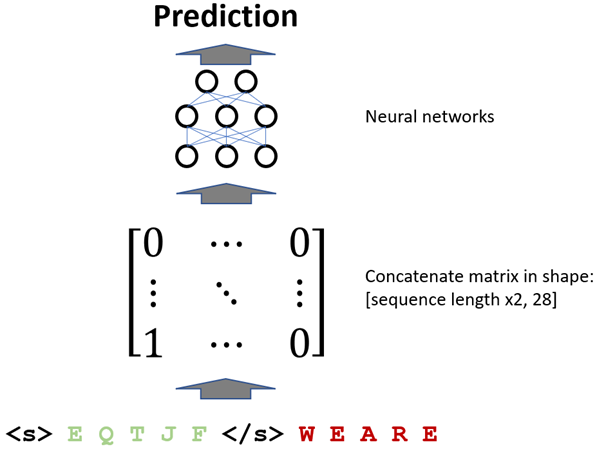
\includegraphics[width=0.5\linewidth]{myReport//figures/input_seq.png}
    \caption{Input the features into network by sequences}
    \label{fig:enter-label}
\end{figure}

\noindent\textbf{Sequential inputs} \qquad		There are two different methods to feed the pair of ciphertext and plaintext into the neural network. The first method is similar with the method that use by Greydanus \cite{greydanus2017learning} for cipher learning which is adding the ciphertext and plaintext into a single text. In this implementation, we construct a dictionary that contains each alphabet and two special tokens. Each token is fed into the network in the form of one-hot encoding. An input sequence could be represented as a matrix in shape [sequence length, dictionary size]. For example, in the example above we input a plaintext and a ciphertext of length of 5. The shape of the matrix would be [12, 28]. The first-dimension length is 12 because the input sequence contains the plaintext, ciphertext and two special tokens. The second dimension is 28 because the dictionary contains 26 English letters and 2 special tokens. During mini-batched training, the matrix would have an additional dimension for the stack of batches [sequence length, batch size, dictionary size]. For example, if we set the batch size to 1800, the shape of the matrix would be [12, 1800, 28].

\begin{figure}[hbt!]
    \centering
    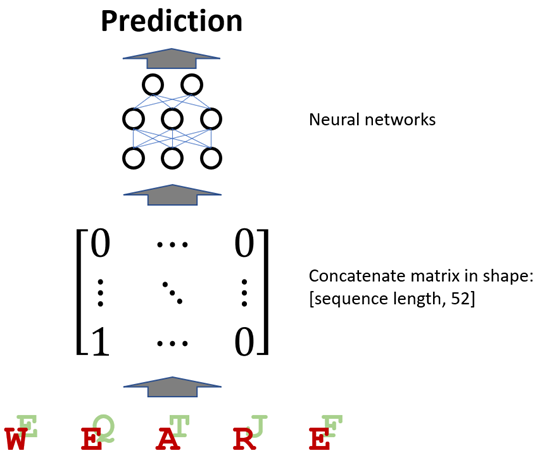
\includegraphics[width=0.5\linewidth]{myReport//figures/input_pair.png}
    \caption{Input features into network by paired dataset}
    \label{fig:enter-label}
\end{figure}

Concatenated inputs	Another improved method was also mentioned by Greydanus \cite{greydanus2017learning} at the end of key recovery section. It concatenates the one-hot encoding of plaintext and ciphertext together. This method does not require special tokens to divide our input text and each character is fed in pairs. The shape of the matrix in this method is [5, 52]. The length of first dimension length is 5 because each token contains the combined information of ciphertext and plaintext alphabets. Second dimension’s length is 52 because we concatenate two one-hot encoding in length 26. This method is proven to have better performance in converging speed and accuracy. We assume the reason is in the first method, a long text doesn’t contain the information of symmetry between ciphertext and plaintext. In the second method, the symmetry between ciphertext and plaintext is given, so the network is not required to learn the symmetry. Another significant feature of concatenated input is it allows us to make a token-wise prediction. We will illustrate the details of the prediction in the next part.


\section{Prediction}

\begin{figure}[hbt!]
    \centering
    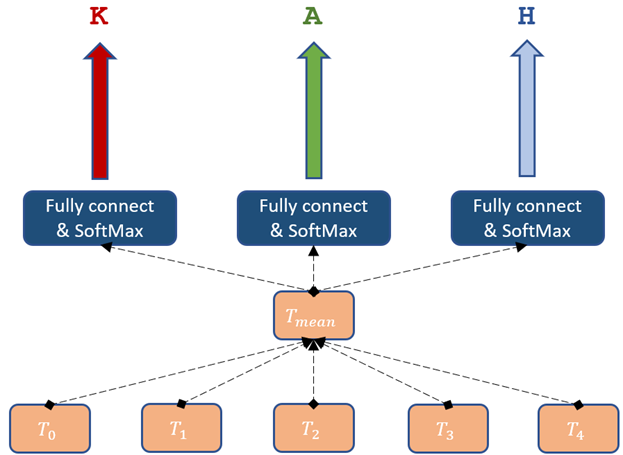
\includegraphics[width=0.5\linewidth]{myReport//figures/output_proj.png}
    \caption{An alternative output method}
    \label{fig:enter-label}
\end{figure}

\noindent\textbf{Pair-wise prediction} \qquad		What pair-wise prediction does is make a position prediction for each token from inputs. This method is also illustrated at the top of \textbf{Figure 3.6}. In Enigma machine, the encryption keeps changing depending on the time series. The next character is encrypted by the rotor position that is one step ahead from the current position. Based on this fact, we can train the network to make predictions for each time step. The implementation is using three different linear projectors to predict the position of the first, second and third rotor. We already seen the output in Figure \textbf{Figure 3.3}. The shape of output from LSTM and Transformer encoder is [sequence length, batch size, features]. The number of output channels in each linear projector is 26, for the prediction of position. The prediction output would be a matrix in shape [rotors, sequence length, batch size, 26]. We applied a SoftMax activation function to the final dimension to obtain the index prediction of position.

\noindent\textbf{Global prediction} \qquad		Another method of prediction is only to predict the initial state based on the entire output. We could compute the average of the sequence dimension. The computer result is a matrix in shape [batch size, features], which is used for a linear projector to predict the initial state of three rotors. This method has less performance on the converging and results but it’s flexible and could be applied on a cipher with different length of ciphertext and plaintext.

\section{Optimization}
\noindent\textbf{Loss function} \qquad	We optimise the model by compute the categorical cross entropy loss on predictions and targets. This loss function is also named as SoftMax loss or Cross Entropy loss in PyTorch’s documentation, which is different from the binary cross entropy loss. For a vector with length j. The term of Categorical cross entropy loss is:

\begin{center}
\(L_\text{CCE} (\hat{y}, y)= -  \hat{y_i}log(〖Softmax(y ̂)〗_i )\)
\end{center}


Where the y ̂ is the prediction score from entire minibatch, i is the index of target categories. In our training task, this is referred to the 26 different positions of Rotors. By minimize this loss function, the score of target positions would be maximize. 

\noindent\textbf{Hyperparameters and training strategy} \qquad	The optimizer we use in this project is Adam. We used learning rate 3e-4 because it is a very commonly used learning rate in deep learning task. We set beta 2 to 0.98 following the setting of Transformer paper. Hyperparameters regard to the architecture of neural networks include number of layers for LSTM and Transformer encoder, the dimensions of LSTM and Transformer Encoder, and the number of attention heads in Transformer Encoder. We could also configure the network to only use LSTM or Transformer Encoder. For the dataset, we have the hyperparameters to control the length of input sequences and batch size. In the experiment, we keep trying each hyperparameter to search for the best parameters setting.

The training strategy we use is warm-up learning rate. He et al \cite{he2016deep} illustrated that using a large learning rate at the beginning would lead to numerical instability. To address this, Goyal et al \cite{he2019bag} propose learning rate warm-up strategy which is linearly increasing the learning rate at the beginning of the training. In practice, we found that using learning rate 3e-4 at the beginning, the network would likely fail to converge because of gradient explode. Warm-up learning rate strategy allow us to train a network with larger learning with stability. This gave the training speed a significant boost.

\section{Metrics and evaluation}
Our measuring on the metric is straight forward. We use accuracy to observe how well the neural network makes predictions. Our evaluation would also focus on how the model could handle input sequences with different length.